% \documentclass[tikz, border=20pt]{standalone}
\documentclass[tikz,border=20pt,convert={outfile=convdemo1.svg, command=\unexpanded{pdf2svg \infile\space\outfile}}]{standalone} % pdflatex --shell-escape convdemo1.tex 
\renewcommand{\familydefault}{\sfdefault}

\usepackage{amsmath}
\usetikzlibrary{positioning, arrows.meta, backgrounds, matrix}

\begin{document}
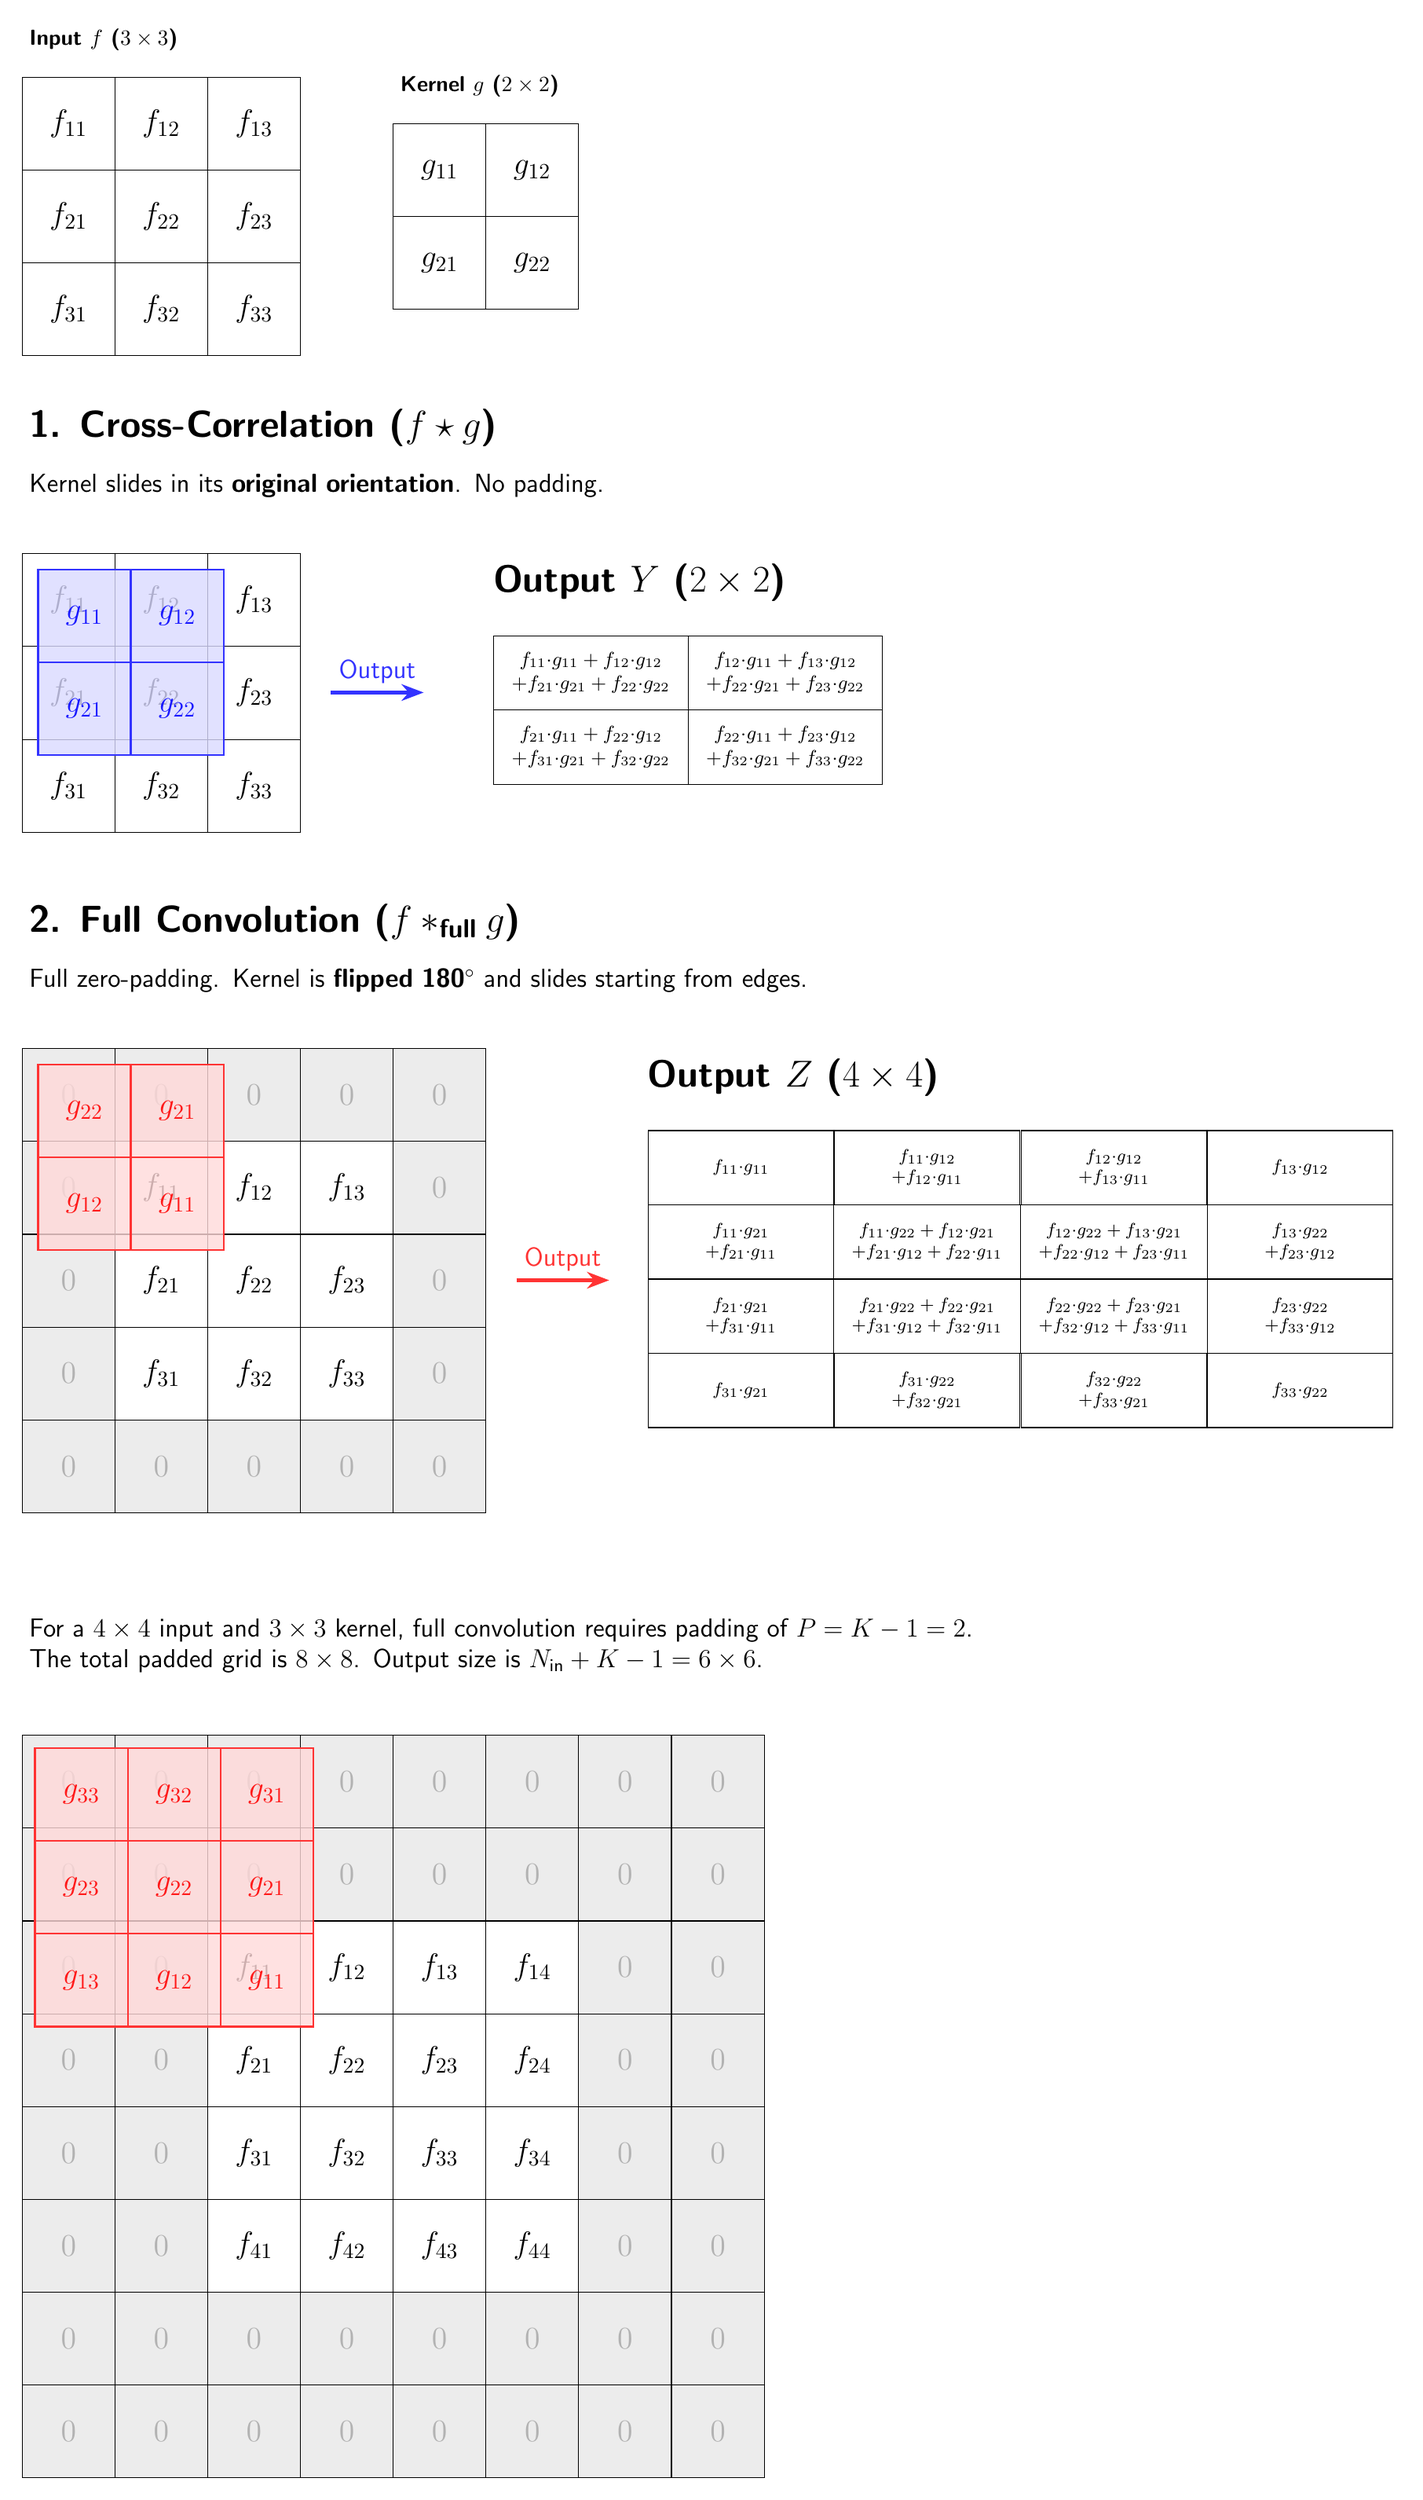
\begin{tikzpicture}[
    >=Stealth,
    cell/.style={draw, minimum size=1.5cm, font=\Large, align=center},
    pad/.style={draw, minimum size=1.5cm, font=\Large, fill=gray!15, text=gray!60, align=center},
    kcell/.style={draw=blue!80, thick, fill=blue!15, fill opacity=0.8, text opacity=1, minimum size=1.5cm, font=\Large\bfseries, text=blue!90, align=center},
    fcell/.style={draw=red!80, thick, fill=red!15, fill opacity=0.8, text opacity=1, minimum size=1.5cm, font=\Large\bfseries, text=red!90, align=center}
]

% ==========================================
% 1. ORIGINAL MATRICES
% ==========================================

% Input f (3x3)
\node[font=\normalsize\bfseries, anchor=south west] at (0, 0.3) {Input $f$ ($3 \times 3$)};
\foreach \i in {1,2,3} {
    \foreach \j in {1,2,3} {
        \node[cell, anchor=north west] at (\j*1.5 - 1.5, -\i*1.5 + 1.5) {$f_{\i\j}$};
    }
}

% Kernel g (2x2)
\begin{scope}[shift={(6, -0.75)}]
    \node[font=\normalsize\bfseries, anchor=south west] at (0, 0.3) {Kernel $g$ ($2 \times 2$)};
    \foreach \i in {1,2} {
        \foreach \j in {1,2} {
            \node[cell, anchor=north west] at (\j*1.5 - 1.5, -\i*1.5 + 1.5) {$g_{\i\j}$};
        }
    }
\end{scope}

% ==========================================
% 2. 2D CROSS-CORRELATION
% ==========================================
\begin{scope}[shift={(0, -6.5)}]
    \node[font=\LARGE\bfseries, anchor=south west] at (0, 0.4) {1. Cross-Correlation ($f \star g$)};
    \node[font=\large, anchor=north west, text width=12cm] at (0, 0.2) { Kernel slides in its \textbf{original orientation}. No padding.};

    \begin{scope}[shift={(0, -1.2)}]
        % Base Input f
        \foreach \i in {1,2,3} {
            \foreach \j in {1,2,3} {
                \node[cell, anchor=north west] at (\j*1.5 - 1.5, -\i*1.5 + 1.5) {$f_{\i\j}$};
            }
        }
        
        % Overlaid Kernel g (Offset for visual clarity)
        \begin{scope}[shift={(0.25, -0.25)}]
            \foreach \i in {1,2} {
                \foreach \j in {1,2} {
                    \node[kcell, anchor=north west] at (\j*1.5 - 1.5, -\i*1.5 + 1.5) {$g_{\i\j}$};
                }
            }
        \end{scope}
        
        % Sliding Arrow
        \draw[->, blue!80, ultra thick] (5.0, -2.25) -- ++(1.5, 0) node[midway, above, font=\large] {Output};

        % Explicit Output Matrix Y (2x2)
        \begin{scope}[shift={(7.5, -1.2)}]
            \node[font=\LARGE\bfseries, anchor=south west] at (0, 0.3) {Output $Y$ ($2 \times 2$)};
            \matrix[matrix of math nodes, nodes={draw, minimum height=1.2cm, minimum width=3cm, font=\small}, row sep=-\pgflinewidth, column sep=-\pgflinewidth, anchor=north west] at (0,0) {
                \begin{array}{c} f_{11}{\cdot}g_{11} + f_{12}{\cdot}g_{12} \\ + f_{21}{\cdot}g_{21} + f_{22}{\cdot}g_{22} \end{array} &
                \begin{array}{c} f_{12}{\cdot}g_{11} + f_{13}{\cdot}g_{12} \\ + f_{22}{\cdot}g_{21} + f_{23}{\cdot}g_{22} \end{array} \\
                \begin{array}{c} f_{21}{\cdot}g_{11} + f_{22}{\cdot}g_{12} \\ + f_{31}{\cdot}g_{21} + f_{32}{\cdot}g_{22} \end{array} &
                \begin{array}{c} f_{22}{\cdot}g_{11} + f_{23}{\cdot}g_{12} \\ + f_{32}{\cdot}g_{21} + f_{33}{\cdot}g_{22} \end{array} \\
            };
        \end{scope}
    \end{scope}
\end{scope}

% ==========================================
% 3. 2D FULL CONVOLUTION
% ==========================================
\begin{scope}[shift={(0, -14.5)}]
    \node[font=\LARGE\bfseries, anchor=south west] at (0, 0.4) {2. Full Convolution ($f \ast_{\text{full}} g$)};
    \node[font=\large, anchor=north west, text width=20cm] at (0, 0.2) {Full zero-padding. Kernel is \textbf{flipped 180$^\circ$} and slides starting from edges.};

    \begin{scope}[shift={(0, -1.2)}]
        % Outer Padding Layer (Only drawing the perimeter, preventing overlaps)
        % Top and bottom rows (i = 1 and 5)
        \foreach \i in {1, 5} {
            \foreach \j in {1,...,5} {
                \node[pad, anchor=north west] at (\j*1.5 - 1.5, -\i*1.5 + 1.5) {$0$};
            }
        }
        % Left and right columns (middle rows i = 2, 3, 4 and columns j = 1, 5)
        \foreach \i in {2, 3, 4} {
            \foreach \j in {1, 5} {
                \node[pad, anchor=north west] at (\j*1.5 - 1.5, -\i*1.5 + 1.5) {$0$};
            }
        }
        
        % Inner Input f (3x3)
        \foreach \i/\frow in {2/1, 3/2, 4/3} {
            \foreach \j/\fcol in {2/1, 3/2, 4/3} {
                \node[cell, anchor=north west] at (\j*1.5 - 1.5, -\i*1.5 + 1.5) {$f_{\frow\fcol}$};
            }
        }
        
        % Overlaid Flipped Kernel (Starts at top-left of padding)
        \begin{scope}[shift={(0.25, -0.25)}]
            \node[fcell, anchor=north west] at (1*1.5 - 1.5, -1*1.5 + 1.5) {$g_{22}$};
            \node[fcell, anchor=north west] at (2*1.5 - 1.5, -1*1.5 + 1.5) {$g_{21}$};
            \node[fcell, anchor=north west] at (1*1.5 - 1.5, -2*1.5 + 1.5) {$g_{12}$};
            \node[fcell, anchor=north west] at (2*1.5 - 1.5, -2*1.5 + 1.5) {$g_{11}$};
        \end{scope}
        
        % Sliding Arrow
        \draw[->, red!80, ultra thick] (8.0, -3.75) -- ++(1.5, 0) node[midway, above, font=\large] {Output};

        % Explicit Output Matrix Z (4x4)
        \begin{scope}[shift={(10.0, -1.2)}]
            \node[font=\LARGE\bfseries, anchor=south west] at (0, 0.3) {Output $Z$ ($4 \times 4$)};
            \matrix[matrix of math nodes, nodes={draw, minimum height=1.2cm, minimum width=3cm, font=\footnotesize}, row sep=-\pgflinewidth, column sep=-\pgflinewidth, anchor=north west] at (0,0) {
                f_{11}{\cdot}g_{11} &
                \begin{array}{c} f_{11}{\cdot}g_{12} \\ + f_{12}{\cdot}g_{11} \end{array} &
                \begin{array}{c} f_{12}{\cdot}g_{12} \\ + f_{13}{\cdot}g_{11} \end{array} &
                f_{13}{\cdot}g_{12} \\
                \begin{array}{c} f_{11}{\cdot}g_{21} \\ + f_{21}{\cdot}g_{11} \end{array} &
                \begin{array}{c} f_{11}{\cdot}g_{22} + f_{12}{\cdot}g_{21} \\ + f_{21}{\cdot}g_{12} + f_{22}{\cdot}g_{11} \end{array} &
                \begin{array}{c} f_{12}{\cdot}g_{22} + f_{13}{\cdot}g_{21} \\ + f_{22}{\cdot}g_{12} + f_{23}{\cdot}g_{11} \end{array} &
                \begin{array}{c} f_{13}{\cdot}g_{22} \\ + f_{23}{\cdot}g_{12} \end{array} \\
                \begin{array}{c} f_{21}{\cdot}g_{21} \\ + f_{31}{\cdot}g_{11} \end{array} &
                \begin{array}{c} f_{21}{\cdot}g_{22} + f_{22}{\cdot}g_{21} \\ + f_{31}{\cdot}g_{12} + f_{32}{\cdot}g_{11} \end{array} &
                \begin{array}{c} f_{22}{\cdot}g_{22} + f_{23}{\cdot}g_{21} \\ + f_{32}{\cdot}g_{12} + f_{33}{\cdot}g_{11} \end{array} &
                \begin{array}{c} f_{23}{\cdot}g_{22} \\ + f_{33}{\cdot}g_{12} \end{array} \\
                f_{31}{\cdot}g_{21} &
                \begin{array}{c} f_{31}{\cdot}g_{22} \\ + f_{32}{\cdot}g_{21} \end{array} &
                \begin{array}{c} f_{32}{\cdot}g_{22} \\ + f_{33}{\cdot}g_{21} \end{array} &
                f_{33}{\cdot}g_{22} \\
            };
        \end{scope}
    \end{scope}

    % Flipped Kernel Reference Graphic
    % \begin{scope}[shift={(2.25, -9.5)}]
    %     \node[font=\Large\bfseries, anchor=south west, text=red!80] at (0, 0.3) {Flipped Kernel Reference};
    %     \node[fcell, fill opacity=0.1, anchor=north west] at (0, 0) {$g_{22}$};
    %     \node[fcell, fill opacity=0.1, anchor=north west] at (1.5, 0) {$g_{21}$};
    %     \node[fcell, fill opacity=0.1, anchor=north west] at (0, -1.5) {$g_{12}$};
    %     \node[fcell, fill opacity=0.1, anchor=north west] at (1.5, -1.5) {$g_{11}$};
        
    %     % Rotation indication
    %     \node[font=\large, text=gray, align=center, anchor=south] at (1.5, 0.8) {Rotated 180$^\circ$ \\ ($H$ \& $V$ flip)};
    % \end{scope}
\end{scope}

\begin{scope}[shift={(0, -25)}]
    % \node[font=\LARGE\bfseries, anchor=south west] at (0, 0.4) {Full Convolution ($f \ast_{\text{full}} g$)};
    \node[font=\large, anchor=north west, text width=16cm] at (0, 0.2) {For a $4 \times 4$ input and $3 \times 3$ kernel, full convolution requires padding of $P = K - 1 = 2$. \\ The total padded grid is $8 \times 8$. Output size is $N_{\text{in}} + K - 1 = 6 \times 6$.};

    \begin{scope}[shift={(0, -1.8)}]
        
        % --------------------------------------
        % Optimized Outer Padding Layer (8x8 grid)
        % --------------------------------------
        % Top 2 rows (i = 1, 2)
        \foreach \i in {1, 2} {
            \foreach \j in {1,...,8} {
                \node[pad, anchor=north west] at (\j*1.5 - 1.5, -\i*1.5 + 1.5) {$0$};
            }
        }
        % Bottom 2 rows (i = 7, 8)
        \foreach \i in {7, 8} {
            \foreach \j in {1,...,8} {
                \node[pad, anchor=north west] at (\j*1.5 - 1.5, -\i*1.5 + 1.5) {$0$};
            }
        }
        % Left 2 columns (rows i = 3, 4, 5, 6 | cols j = 1, 2)
        \foreach \i in {3, 4, 5, 6} {
            \foreach \j in {1, 2} {
                \node[pad, anchor=north west] at (\j*1.5 - 1.5, -\i*1.5 + 1.5) {$0$};
            }
        }
        % Right 2 columns (rows i = 3, 4, 5, 6 | cols j = 7, 8)
        \foreach \i in {3, 4, 5, 6} {
            \foreach \j in {7, 8} {
                \node[pad, anchor=north west] at (\j*1.5 - 1.5, -\i*1.5 + 1.5) {$0$};
            }
        }
        
        % --------------------------------------
        % Inner Input f (4x4)
        % --------------------------------------
        Resides in rows 3-6 and cols 3-6
        \foreach \i/\frow in {3/1, 4/2, 5/3, 6/4} {
            \foreach \j/\fcol in {3/1, 4/2, 5/3, 6/4} {
                \node[cell, anchor=north west] at (\j*1.5 - 1.5, -\i*1.5 + 1.5) {$f_{\frow\fcol}$};
            }
        }
        
        % --------------------------------------
        % Overlaid Flipped Kernel (Starts at top-left)
        % --------------------------------------
\begin{scope}[shift={(0.2, -0.2)}]
            \foreach \i/\vi in {1/3, 2/2, 3/1} {
                \foreach \j/\vj in {1/3, 2/2, 3/1} {
                    \node[fcell, anchor=north west] at (\j*1.5 - 1.5, -\i*1.5 + 1.5) {$g_{\vi\vj}$};
                }
            }
        \end{scope}
        
        % --------------------------------------
        % Sliding Arrow
        % --------------------------------------
        % \draw[->, red!80, ultra thick] (10.0, -4.8) -- ++(1.5, 0) node[midway, above, font=\large] {Output};

        % --------------------------------------
        % Output Matrix Z (6x6)
        % --------------------------------------
        % \begin{scope}[shift={(12.0, -1.2)}]
        %     \node[font=\LARGE\bfseries, anchor=south west] at (0, 0.4) {Output $Z$ ($6 \times 6$)};
        %     \foreach \i in {1,...,6} {
        %         \foreach \j in {1,...,6} {
        %             \node[cell, anchor=north west] at (\j*1.2 - 1.2, -\i*1.2 + 1.2) {$Z_{\i\j}$};
        %         }
        %     }
        % \end{scope}
        
    \end{scope}
\end{scope}


\end{tikzpicture}
\end{document}